\documentclass[12pt]{article}
\topmargin -0.7in
\oddsidemargin -0.21in
\evensidemargin -0.21in
\textwidth=17cm
\textheight=24cm

\usepackage[utf8]{inputenc}
\usepackage[T2A]{fontenc} 
\usepackage[russian]{babel}
\usepackage{amsmath}
\usepackage{comment}

\usepackage{tikz}
\usepackage{graphicx}
\graphicspath{{./src/}}
\DeclareGraphicsExtensions{.png}

\renewcommand{\l}{\left( }
\renewcommand{\r}{\right) }
\renewcommand{\phi}{\varphi}
\newcommand{\pd}{\partial}
\newcommand{\br}[1]{\l {#1} \r}
\newcommand{\rint}{\int\limits_{-\infty}^{+\infty}}
\newcommand{\pint}{\int\limits_{-\pi}^{\pi}}
\newcommand{\jacobian}[2]{\frac{\pd \br{#1}}{\pd \br{#2}}}
\newcommand{\abs}[1]{\left| #1 \right|}

\def\Dphi{\Delta\phi}
\def\Dy{\Delta y}
\def\Dn{\Delta \eta}
\def\kx{k_x}
\def\kxx{k_x^2}
\def\ky{k_y}
\def\kyy{k_y^2}
\def\kz{k_z}
\def\kzz{k_z^2}
\def\f{\Phi}
\def\y{Y}
\def\d#1#2{\frac{\partial #1}{\partial #2}}
\def\df#1#2#3{\frac{\partial #1}{\partial #2}\Big|_{ #3}}
\def\dff#1#2#3#4{\frac{\partial #1 \left( #2 \right)}{\partial #3}}
\def\ra{\rightarrow}
\def\det#1#2{\frac{D \left( #1 \right)}{D \left( #2 \right)}}
\def\pa{\kx, \kz}
\def\pb{x, \kz}
\def\pc{x, Y}
\def\pd{\f, Y}
\def\pe{\Dphi, \Dy}

\begin{document}

\begin{center}
\large{ПРАВИТЕЛЬСТВО РОССИЙСКОЙ ФЕДЕРАЦИИ} \\
\vspace{2em}
\large{ФЕДЕРАЛЬНОЕ ГОСУДАРСТВЕННОЕ БЮДЖЕТНОЕ ОБРАЗОВАТЕЛЬНОЕ УЧРЕЖДЕНИЕ ВЫСШЕГО ПРОФЕССИОНАЛЬНОГО ОБРАЗОВАНИЯ \\
<<САНКТ-ПЕТЕРБУРГСКИЙ ГОСУДАРСТВЕННЫЙ УНИВЕРСИТЕТ>>\\
(СПбГУ)\\}
Кафедра физики высоких энергий и элементарных частиц\\
Направление <<Физика>>
\end{center}
\begin{figure}[h!]
\center

\includegraphics[width=.25\textwidth,clip]{eagle2.png}
\end{figure}

\begin{center}
\large{\bf ФРАГМЕНТАЦИЯ ЦВЕТНОЙ СТРУНЫ И БЛИЖНИЕ БЫСТРОТНЫЕ КОРРЕЛЯЦИИ ВО ВЗАИМОДЕЙСТВИЯХ АДРОНОВ ВЫСОКИХ ЭНЕРГИЙ}
\end{center}
$$$$
$$$$
\begin{flushright}
Выпускная квалификационная работа студента
$$$$
{\bf Кравцова Павла Сергеевича} \\
\vspace{2em}
Научный руководитель: \\
д.ф.-м.н., проф. {\bf Вечернин В. В.} \\
\vspace{2em}
Рецензент: \\
к.ф.-м.н., ассистент {\bf Мацкевич Е.Е.} \\
\end{flushright}
$$$$

\begin{center}
\Large{
Санкт--Петербург \\
2018}
\end{center}
\thispagestyle{empty}
\newpage

\tableofcontents
\newpage

\section{Введение}
\qquad В адронных столкновениях типа протон-протон при сверх высоких энергиях образуется множество частиц основная часть из которых - $\pi$-мезоны. Считается, что процесс происходит через промежуточное состояние - кварк-глюонную плазму. После остывания плазмы из нее образуются частицы, многие из которых распадаются не успевая долететь до детекторов.
Известно, что порядка 70\% задетектированных заряженных $\pi$-мезонов получаются от распада первичных $\rho$-мезонов по сильному взаимодействию. Данная работа описывает влияние подобных распадов на распределение $\pi$-мезонов по направлениям разлета, в частности на распределение двухчастичных корреляций ($\Dphi$, $\Dy$).

\subsection{Корреляции ($\Dphi$, $\Dy$)}
\qquad Для описания столкновений при сверхвысоких энергиях удобно использовать специальные переменные. Везде в данной работе будем считать, что ось столкновения протонов сонаправленна с осью $z$. Пусть $\vec p, E$ импульс и энергия образовавшейся частицы. Импульс вдоль оси $z$ принято описывать переменной $$y = \frac{1}{2} ln \frac{E + p_z}{E - p_z},$$ которая называется быстротой в направлении $z$. Для краткости мы будем называть ее просто быстротой. В плоскости перпендикулярной к оси $z$ импульс описывается обычными полярными координатами $(p_\perp, \phi)$, где $p_\perp = \sqrt{p_x^2 + p_y^2},$ а $\phi$ есть угол между проекцией $\vec p$ на эту плоскость и осью $x$. Угол $\phi$ изменяется в пределах от $-\pi$ до $\pi$. Таким образом импульс при известной энергии однозначно описывается тремя переменными $(y, \phi, p_\perp)$. Нас будут интересовать переменные $(y, \phi)$, т. к. они связанны с направлением.

Сами по себе распределения по $(y, \phi)$ мало содержательны. Из азимутальной симметрии эксперимента следует, что распределение образовавшихся частиц по $\phi$ равномерное. Так же из эксперимента известно, что распределение образовавшихся частиц по $y$ приблизительно равномерно в некотором интервале $[y_{min}, y_{max}]$ и равно нулю вне этого интервала. Эти распределения называются одночастичными.

Гораздо сложнее и содержательнее выглядят двухчастичные распределения или двухчастичные корреляции. В них рассматриваются всевозможные пары образовавшихся частиц и их координаты $(\phi_1, \phi_2, y_1, y_2)$. Из сказаного выше ясно что нетривиально могут быть распределены лишь комбинации $\Dphi = \phi_1 - \phi_2, \Dy = y_1 - y_2$. Ниже будут рассматриваться двумерное распределение $(\Dphi, \Dy)$ и влияние на него распадов $\rho$-резонансов.

\subsection{Обозначения}
\qquad Будем обозначать за $\rho_x (a)$ - плотность распределения величины $x$ в точке $x = a$. Если из названия точки сразу ясно по какой величине растределение, индекс будем опускать: $\rho(x) = \rho_x (x)$. Плотность распределения нормирована
$$\rint dx\ \rho (x) = 1,$$
поэтому вычисления достаточно проводить с точностью до множителя, который всегда можно восстановить из условий нормировки.

\subsection{Цель работы}
\qquad Цель работы - найти $\rho(\Dphi, \Dy)$ для двух $\pi$-мезонов, которые образовались из распада $\rho$-мезона летяшего с некоторым импульсом. Как мы увидим в дальнейшем, подобная модель приводит к образованию "вулканообразного"\ пика в точке $\Dphi = 0, \Dy = 0$. Данный пик действительно наблюдается в различных экспериментальных данных (например в \cite{exp_data}).

\section{Вычисления}
\subsection{Постановка задачи}
\qquad Пусть имеется $\rho$-мезон с импульсом $\vec R$ и массой $M$. Он распадается на два $\pi$-мезона с импульсами $\vec p_1, \vec p_2$, массами $m_1 = m_2 = m$ и энергиями $E_1, E_2$.
$$\vec R = \vec p_1 + \vec p_2.$$
$(\phi_1, \phi_2, y_1, y_2)$ - азимутальные углы и быстроты $\pi$-мезонов. Нас интересуют величины
\begin{gather*}
	\Dphi = \phi_1 - \phi_2,\\  
	\Dy = y_1 - y_2.
\end{gather*}

Пусть в системе отсчета центра масс $\rho$-мезона импульсы $\pi$-мезонов равны $\vec k$ и $-\vec k$ соответственно, а энергия каждого из $\pi$-мезонов равна $\varepsilon$. Из закона сохранения энергии
$$2\varepsilon = M.$$
Мы будем считать направление вектора $\vec k$ произвольным и распределенным равномерно. Модуль этого вектора $|\vec k| = k$ выражается через $\varepsilon$: 
$$k = \sqrt {\varepsilon^2 - m^2} = \sqrt{\frac{M^2}{4}-m^2}.$$  

\subsection{Преобразования Лоренца}
\qquad Не умаляя общности можно считать импульс $\vec R$ перпендикулярным оси $z$. Наличие $R_z$ повлияло бы лишь на быстроты $y_1, y_2$. Однако у быстроты есть свойство, что при преобразованиях Лоренца вдоль оси $z$ быстрота изменяется лишь на некоторое слагаемое:
$$y \rightarrow y + C(R_z).$$
Отсюда видно что $\Dy$ инвариантна относительно преобразований Лоренца вдоль оси $z$:
$$\Dy = y_1 - y_2 \rightarrow (y_1 - C(R_z)) - (y_2 - C(R_z)) = y_1 - y_2,$$
и наличие $R_z$ не влияло бы на результат. Аналогично можно считать, что $\vec R$ сонаправлен с осью $x$. Наличие у $\vec R$ ненулевого азимутального угла привело бы лишь к одинаковому сдвигу $\phi_1$ и $\phi_2$, но не повлияло бы на их разность.

В системе отсчета центра масс 4-импульсы всех мезонов:
\begin{gather*}
	\begin{cases}
		\rho-\text{мезон}:\ (M, 0, 0, 0) \\
		\text{первый}\ \pi-\text{мезон}:\ (\varepsilon, k_x, k_y, k_z) \\
		\text{второй}\ \pi-\text{мезон}:\ (\varepsilon, -k_x, -k_y, -k_z) \\
	\end{cases}
\end{gather*}
В тоже время в лобораторной системе отсчета эти имульсы равны:  
\begin{gather*}
	\begin{cases}
		\rho-\text{мезон}:\ (\sqrt{M^2 + R^2}, R, 0, 0) \\
		\text{первый}\ \pi-\text{мезон}:\ (E_1, p_{1x}, p_{1y}, p_{1z}) \\
		\text{второй}\ \pi-\text{мезон}:\ (E_2, p_{2x}, p_{2y}, p_{2z}) \\
	\end{cases}
\end{gather*}

Пусть $V$ - модуль скорости $\rho$-мезона в лабораторной системе отсчета.  
Можно связать импульсы в разных системах отсчета с помощью преобразований Лоренца вдоль оси $x$:
\begin{gather}
	\label{Lorenz1}
	R = \frac{VM}{\sqrt{1 - V^2}}
\end{gather}
\begin{gather}
	\label{Lorenz2}
	\begin{cases}
		E_1 = \frac{V k_x + \varepsilon}{\sqrt{1 - V^2}} \\
		p_{1x} = \frac{k_x + V\varepsilon}{\sqrt{1 - V^2}} \\
		p_{1y} = k_y \\
		p_{1z} = k_z \\
	\end{cases}
	\begin{cases}
		E_2 = \frac{-V k_x + \varepsilon}{\sqrt{1 - V^2}} \\
		p_{2x} = \frac{-k_x + V\varepsilon}{\sqrt{1 - V^2}} \\
		p_{2y} = -k_y \\
		p_{2z} = -k_z \\
	\end{cases}
\end{gather}
Из уравнения (\ref{Lorenz1}) можно получить модуль скорости: $V = \sqrt\frac{R^2}{R^2 + M^2}$ и подставить его в (\ref{Lorenz2}).

\subsection{Выражения для $\Dphi$ и $\Dy$}
\qquad
У нас есть переменные $k_x, k_y, k_z,$ про которые известно как они распределенны. Для того чтобы найти распределение $\rho(\Dphi, \Dy)$ необходимо связать переменные $\Dphi, \Dy$ с $k_x, k_y, k_z$. Выразим энергии и декартовы координаты импульсов $\pi$-мезонов через $k_x, k_y, k_z$:
\begin{gather}
	\begin{cases}
		E_1 = a M / 2 + k_x R / M \\
		p_{1x} = R / 2 + a k_x \\
		p_{1y} = k_y \\
		p_{1z} = k_z \\
	\end{cases}
	\begin{cases}
		E_2 = a M / 2 - k_x R / M \\
		p_{2x} = R / 2 - a k_x \\
		p_{2y} = -k_y \\
		p_{2z} = -k_z \\
	\end{cases}
\end{gather}
Здесь введено обозначение
\begin{gather}
	a = \frac{\sqrt{M^2 + R^2}}{M} = \sqrt{1 + \frac{R^2}{M^2}}.  
\end{gather}
Выразим азимуты и быстроты вдоль оси $z$ $\pi$-мезонов через $k_x, k_y, k_z$:
\begin{gather}
	\begin{cases}
		tg\ \phi_1 = \frac{p_{1y}}{p_{1x}} = \frac{k_y}{R / 2 + a k_x} \\
		tg\ \phi_2 = \frac{p_{2y}}{p_{2x}} = -\frac{k_y}{R / 2 - a k_x} \\
		y_1 = \frac{1}{2} ln \frac{E_1 + p_{1z}}{E_1 - p_{1z}} = \frac{1}{2} ln \frac{E_1 + k_z}{E_1 - k_z} \\
		y_2 = \frac{1}{2} ln \frac{E_2 + p_{2z}}{E_2 - p_{2z}} = \frac{1}{2} ln \frac{E_2 - k_z}{E_2 + k_z} \\
	\end{cases}
\end{gather}
Интересующие нас величины
\begin{gather}
\label{tg}
tg \Dphi = \frac{R k_y}{R^2 / 4 - a^2 k_x^2 - k_y^2} = \frac{\pm R\sqrt{k^2 - k_x^2 - k_z^2}}{R^2 / 4 - k^2 - k_x^2 R^2 / M^2 + k_z^2}
\end{gather}
\begin{gather}
\label{dy}
\Dy = \frac{1}{2} ln \frac{(E_1 + \kz)(E_2 + \kz)}{(E_1 - \kz)(E_2 - \kz)} = \frac{1}{2} ln \frac{(R^2 + M^2) / 4 - \kxx R^2 / M^2 + \kzz +\kz \sqrt{R^2 + M^2}}{(R^2 + M^2) / 4 - \kxx R^2 / M^2 + \kzz -\kz \sqrt{R^2 + M^2}}
\end{gather}

\subsection{Распределение $\rho(\kx, \kz)$}
\qquad Распределение $\rho(\kx, \ky, \kz)$- это равномерное распределение на сфере $\kxx + \kyy + \kzz = k^2$, что означает
$$\rho(\kx, \ky, \kz) \propto \delta(\kxx + \kyy + \kzz - k^2).$$
Можно избавиться от дельта-функции, рассматривая распределение $\rho(\kx, \kz)$:
$$ \rho(\kx, \kz) = \rint d\ky \rho(\kx, \ky, \kz) \propto  \rint d\ky \delta(\kxx + \kyy + \kzz - k^2) \propto \frac{1}{\sqrt{\kxx + \kzz}}$$
Такое преобразование возможно для наших целей, т. к. в нащей задачи знак $\ky$ не влияет на результат. В общем случае варианты $\ky = \sqrt{\kxx + \kzz}$ и $\ky = -\sqrt{\kxx + \kzz}$ необходимо рассматривать раздельно.

\subsection{Замены переменных}
\qquad Мы сделаем следующие замены переменных:
\begin{gather}
\label{chain}
\pa\ra\pb\ra\pc\ra\pd\ra\pe
\end{gather}

Переменные выражаются друг через друга следующим образом:
\begin{gather}
	\label{rep1}
	x = \kxx R^2 / M^2  + k^2 - \kzz - R^2 / 4
\end{gather}
\begin{gather}
	\label{rep2}
	\y = \frac{k^2 + M^2/4 - x + \kz \sqrt{R^2 + M^2}}{k^2 + M^2/4 - x - \kz \sqrt{R^2 + M^2}}
\end{gather}
\begin{gather}
	\label{rep3}
	\f =  \mp \frac{1}{x}\sqrt{(R^2 + M^2)k^2 - u^2 (k^2 + M^2 / 4 - x)^2 - M^2 x - M^2 R^2 / 4}
\end{gather}
\begin{gather}
	\label{rep4}
	\Dphi = arctg\f
\end{gather}	
\begin{gather}
	\label{rep5}
	\Dy = \frac{1}{2} ln \y
\end{gather}

Нам так же понадобятся обратные преобразования:
\begin{gather}
	\label{arep1}
	\kx = \frac{M^2}{R^2} (x + \kzz + R^2 / 4 - k^2)
\end{gather}
\begin{gather}
	\label{arep2}
	\kz = \frac{\y - 1}{\y + 1}\frac{k^2 + M^2 / 4 - x}{\sqrt{R^2 + M^2}} = u \frac{k^2 + M^2 / 4 - x}{\sqrt{R^2 + M^2}}
\end{gather}
\begin{gather}
	\label{arep3}
	x =  \frac{-(M^2 / 2 + u^2 m^2) + \sqrt{(M^2 / 2 + u^2 m^2)^2 - (\f^2 + u^2)(m^2(R^2 + M^2) + m^4 u^2 - M^4 / 4)}}{\f^2 + u^2},
\end{gather}
\begin{gather}
	\label{arep4}
	\f = tg \Dphi
\end{gather}	
\begin{gather}
	\label{arep5}
	\y = e^{2\Dy}
\end{gather}
Здесь введена переменная $u$ для сокращения формул:
$$ u = \frac{\y - 1}{\y + 1}.$$
\subsection{Области определения и неодназначность переменных}
\qquad Очевидно ответ не должен зависеть от знака $\Dphi$ так как в задаче имеется зеркальная симметрия. Поэтому достаточно выполнить расчеты в области $\Delta \phi > 0$ и отразить ответ:
$$\rho (-\Dphi, \Dy) = \rho (\Dphi, \Dy)$$
Таким образом можно фиксировать знак в (\ref{rep3}).

Замена (\ref{rep1}) не взаимно-однозначна, так что необходимо выполнять вычисления отдельно для $\kx > 0$ и $\kx < 0$. Тем не менее т. к. в (\ref{tg}, \ref{dy}) $\kx$ входит лишь через $\kxx$, то для обоих вариантов ответ получится одинаковый, поэтому достаточно рассмотреть лишь случай $\kx > 0$ (это уже использованно в (\ref{arep1})). Аналогичные замечания относятся и к (\ref{rep3}). Выше перечисленны и учтены всевозможные неодназначности и теперь рассматриваемую область изменнения переменных можно считать изменяющейся взаимно-однозначно при преобразованиях (\ref{chain}). 

Переменные $\kx, \kz$ изменяются в круге $\kxx + \kzz \le k^2$. При преобразованиях (\ref{chain}) область изменяется как показано на рис. \ref{areas1} - \ref{areas5}. Изображения сгенерированы методом Монте-Карло.

\begin{figure}
	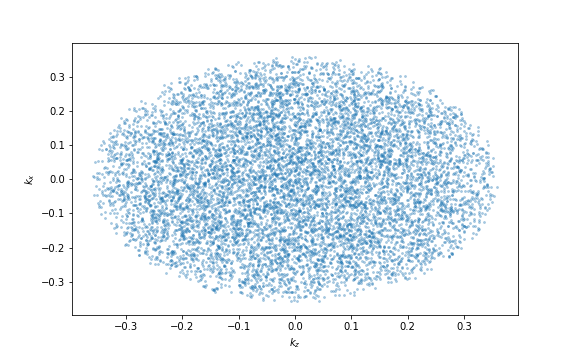
\includegraphics[width=1\linewidth]{1}
	\caption{Область определения $\pa$}
	\label{areas1}
\end{figure}
\begin{figure}
	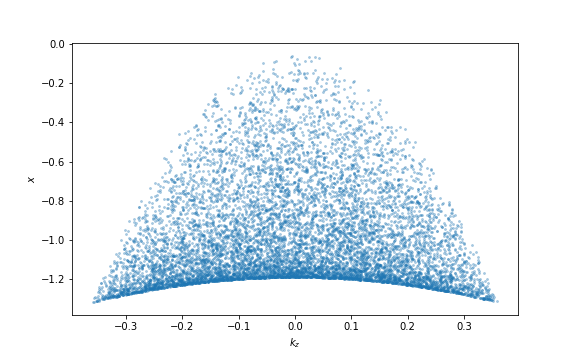
\includegraphics[width=1\linewidth]{2}
	\caption{Область определения $\pb$}
\end{figure}
\begin{figure}
	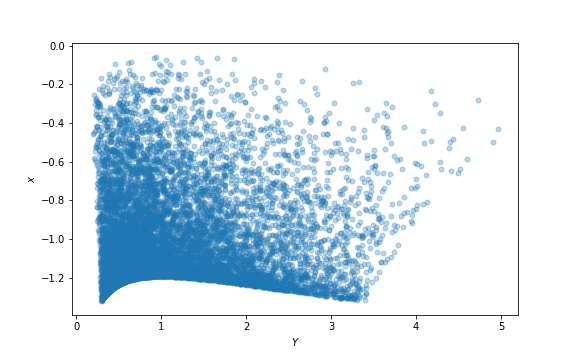
\includegraphics[width=1\linewidth]{3}
	\caption{Область определения $\pc$}
\end{figure}
\begin{figure}
	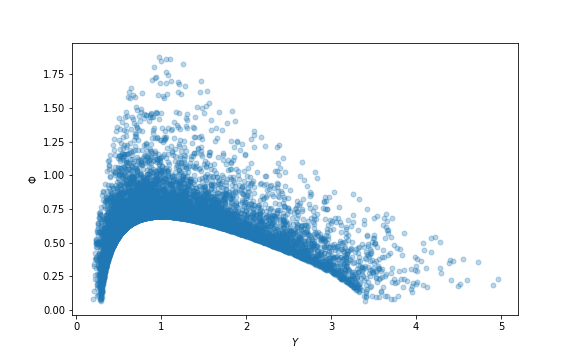
\includegraphics[width=1\linewidth]{4}
	\caption{Область определения $\pd$}
\end{figure}
\begin{figure}
	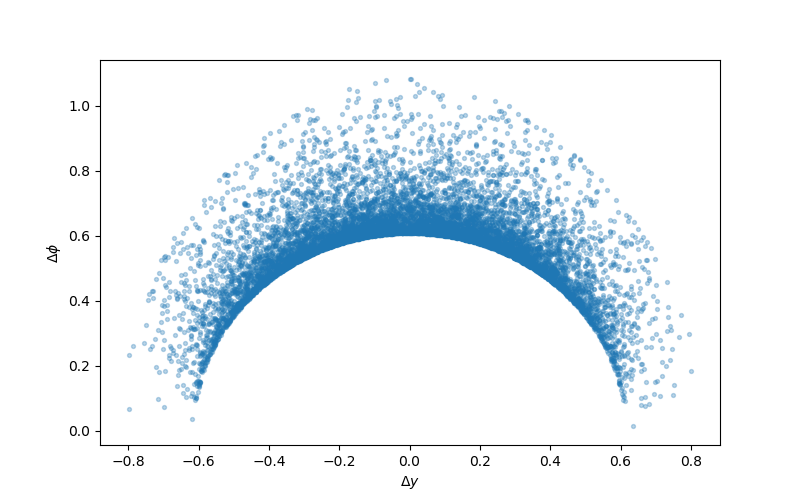
\includegraphics[width=1\linewidth]{5}
	\caption{Область определения $\pe$}
	\label{areas5}
\end{figure}

\subsection{Вычисление $\rho(\Dphi, \Dy)$}
\qquad Распределение $\rho(\Dphi, \Dy)$ получается из $\rho(\kx, \kz)$ заменой переменных, следовательно:
\begin{gather}
\rho(\Dphi, \Dy) = \det{\Dphi, \Dy}{\kx,\kz} \rho(\kx, \kz) \propto \det{\kx,\kz}{\Dphi, \Dy} \frac{1}{\sqrt{\kxx + \kzz}}
\end{gather}
Определитель можно вычислить исходя из цепочки (\ref{chain}) и преобразований (\ref{rep1}-\ref{rep5}, \ref{arep1}-\ref{arep5}):
\begin{gather}
\det{\pa}{\pe} = \det{\pa}{\pb}\det{\pb}{\pc}\det{\pc}{\pd}\det{\pd}{\pe} \\
= \dff{\kx}{\pb}{x}{\kz} \cdot \dff{\kz}{\pc}{Y}{x} \cdot \dff{x}{\pd}{\f}{Y} \cdot \dff{\f}{\pe}{\Dphi}{\Dy} \cdot \dff{Y}{\pe}{\Dy}{\Dphi} \\
\dff{\kx}{\pb}{x}{} = \frac{M^2}{2 R^2 \kx} \\
\dff{\kz}{\pc}{Y}{x} = \frac{2}{(\y + 1)^2}\frac{k^2 + M^2 / 4 - x}{\sqrt{R^2 + M^2}} \\
\d{x}{\f} =  -\frac{2 \f}{\f^2 + u^2} \nonumber \\
\cdot \Big( \frac{-(M^2 / 2 + u^2 m^2) \pm \sqrt{(M^2 / 2 + u^2 m^2)^2 - (\f^2 + u^2)(m^2(R^2 + M^2) + m^4 u^2 - M^4 / 4)}}{\f^2 + u^2} \nonumber \\
+ \frac{m^2(R^2 + M^2) + m^4 u^2 - M^4 / 4}{2\sqrt{(M^2 / 2 + u^2 m^2)^2 - (\f^2 + u^2)(m^2(R^2 + M^2) + m^4 u^2 - M^4 / 4)}} \Big) \\
\dff{Y}{\pe}{\Dy}{} = 2 e^{2\Dy} \\
\dff{\f}{\pe}{\Dphi}{} = \frac{1}{ cos^2 \Dphi}.
\end{gather}

\subsection{Графики}
\qquad На Рис. \ref{r1} - \ref{r5} показана результирующая плотность распределения $\rho(\Dphi, \Dy)$. Вокруг точки $\Dphi = 0, \Dy = 0$ образовалось "вулканообразный пик"\ . Радиус "вулкана"\ тем меньше, чем больше $R$.
\begin{figure}
	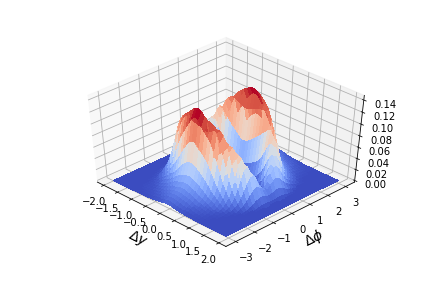
\includegraphics[width=1\linewidth]{R1}
	\caption{Плотность распределения $R = 1\ GeV$}
	\label{r1}
\end{figure}
\begin{figure}
	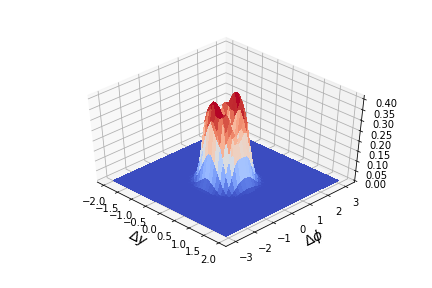
\includegraphics[width=1\linewidth]{R3}
	\caption{Плотность распределения $R = 3\ GeV$}
	\label{r3}
\end{figure}
\begin{figure}
	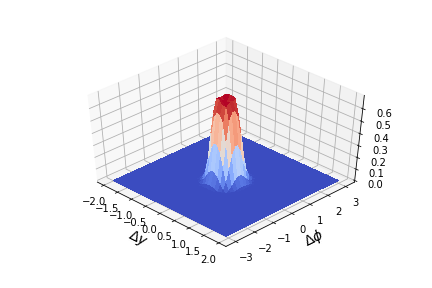
\includegraphics[width=1\linewidth]{R5}
	\caption{Плотность распределения $R = 5\ GeV$}
	\label{r5}
\end{figure}

\section{Связь с другими моделями}
\subsection{Поведение балансной функции $B(\Dn, \Dphi)$}
\qquad Выводы о поведении распределения $\rho(\Dy, \Dphi)$ при наличии резонансов можно эффективно использовать для объяснения поведения так называемой балансной функции $B(\Dn, \Dphi)$. Балансная функция обсуждается, в частности, в \cite{HBT}. Формула (4) из \cite{HBT} вводит определение  $B(\Dn, \Dphi)$:
$$B(\Dn, \Dphi) = \frac{1}{2}[c_{(+,-)} + c_{(-,+)} - c_{(+,+)} - c_{(-,-)}].$$
Величина $\eta$, называемая псевдобыстротой приблизительно равна обычной быстроте $y$. $c_{(+,-)}, c_{(-,+)}, c_{(+,+)}, c_{(-,-)}$ - аналоги распределения $\rho(\Dy, \Dphi)$ для распада на $(\pi_+, \pi_-)$, $(\pi_-, \pi_+)$, $(\pi_+, \pi_+)$, $(\pi_-, \pi_-)$ соответственно. $B(\Dn, \Dphi)$ так же имеет высокий пик в точке $\Dn = 0, \Dphi = 0$. В \cite{HBT} его наличие объясняется квантовыми эффектами, в частности, HBT-корреляцией.

Однако пик можно объяснить и более простым способом, если учесть, что $\rho$-резонанс может распадаться на $(\pi_+, \pi_-)$, но не на $(\pi_+, \pi_+)$ или $(\pi_-, \pi_-)$. Таким образом вклады от $c_{(+,-)}, c_{(-,+)}$ будут большими около точки $\Dn = 0, \Dphi = 0$, при этом они не будут сокращатся вкладами от $c_{(+,+)}, c_{(-,-)}$.

\subsection{Обьединение с моделью одиночной струны}
\begin{figure}
\center{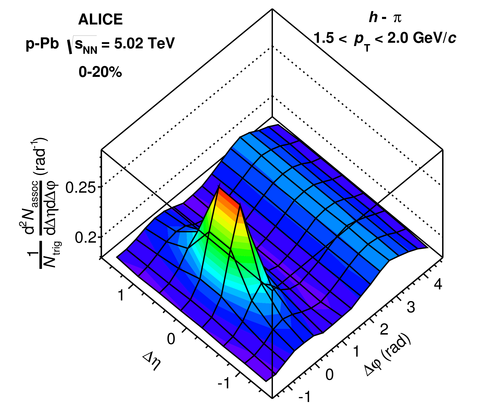
\includegraphics[width=1\textwidth]{exp.png}}
\caption{Экспериментальное распределение числа частиц по $\br{\Delta \eta, \Delta \phi}$ из \cite{exp_data}}
\label{exp}
\end{figure}
\qquad Распределения $\rho (\Dy, \Dphi)$ полученные из эксперимента имеют вид как на Рис. \ref{exp}. Основные его особенности - пик в точке $\Dy = 0, \Dphi = 0$ и "холм"\ на линии $\Dphi = \pi$. Первая особенность объясняется в данной работе, в то время как вторая может быть объяснена в модели адронных струн \cite{model1}-\cite{model4}, в частности корреляцией от соседних фрагментов-источников струны. Это было исследовано нами в работе \cite{bachelor}. В этой работе в аналитическом виде получена форма распределения $\rho' (\Dy, \Dphi)$ для корреляции возникающих при распаде одиночной струны. Общее распределение может быть приблизительно представленно как линейная комбинация этих двух. Таким образом мы имеем достаточно простую модель адекватно приближающюю экспериментальные данные во всей области изменения $(\Dy, \Dphi)$. 

\section{Заключение}
\qquad Была построена модель объясняющая влияние распада $\rho$-резонансов на распределение $\rho (\Dy, \Dphi)$. Модель может использоваться как составная часть более сложных моделей и генераторов событий. В частности, как показано выше она может быть использована при струнном описания адронных столкновений.

Для  $\rho (\Dy, \Dphi)$ удалось найти аналитическую формулу. Она может быть использованна для аппроксимации экспериментальных данных, нахождения параметров столкновения и их погрешностей.

\newpage
\section*{}
\addcontentsline{toc}{section}{Список литературы}
\begin{thebibliography}{00}
\bibitem{exp_data}
{\bf ALICE} Collaboration, B. Abelev \textit{et al.}, arxiv:1307.3237 [nucl-ex].
\bibitem{HBT}
{\bf ALICE} Collaboration, J. Adam \textit{et al.}, Eur. Phys. J. C. (2016) p.76-86
\bibitem{bachelor}
"Двухчастичные корреляции, возникающие при распаде одиночной струны"\ , Кравцов\ П.\ С., Вечернин В. В., выпускная квалификационная работа (2016).
\bibitem{strings}
V. V. Vechernin, Nuclear Physics A 939 (2015) 21-45; arXiv: 1210.7588v2 [hep-ph].
\bibitem{model1}
A. B. Kaidalov, Phys. Lett. B 116, p.459 (1982).
\bibitem{model2}
A. B. Kaidalov, K. A. Ter-Martirosyan, Phys. Lett. B 117 p.247 (1982).
\bibitem{model3}
A. Cappela, U. Sukhatme, Chung-I Tan, J. Tran Thanh Van, Phys. Lett. B 81, 68 (1979).
\bibitem{model4}
A. Cappela, U. Sukhatme, Chung-I Tan, J. Tran Thanh Van, Phys. Rep. 236 p.225 (1994).
\bibitem{fragmentation_lit}
V. V. Vechernin, arXiv: 0812.0604 [hep-ph].
\end{thebibliography}

\end{document}